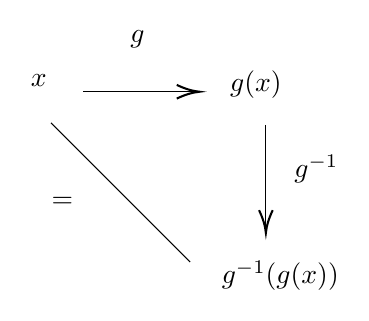
\begin{tikzpicture}[x=0.75pt,y=0.75pt,yscale=-1,xscale=1]
%uncomment if require: \path (0,300); %set diagram left start at 0, and has height of 300

%Straight Lines [id:da6700061600248707] 
\draw    (87.5,98) -- (141.5,98) ;
\draw [shift={(143.5,98)}, rotate = 180] [color={rgb, 255:red, 0; green, 0; blue, 0 }  ][line width=0.75]    (10.93,-3.29) .. controls (6.95,-1.4) and (3.31,-0.3) .. (0,0) .. controls (3.31,0.3) and (6.95,1.4) .. (10.93,3.29)   ;
%Straight Lines [id:da20137743507285333] 
\draw    (175.5,114) -- (175.5,164) ;
\draw [shift={(175.5,166)}, rotate = 270] [color={rgb, 255:red, 0; green, 0; blue, 0 }  ][line width=0.75]    (10.93,-3.29) .. controls (6.95,-1.4) and (3.31,-0.3) .. (0,0) .. controls (3.31,0.3) and (6.95,1.4) .. (10.93,3.29)   ;
%Straight Lines [id:da9015937384996593] 
\draw    (72,113) -- (139,180) ;

% Text Node
\draw (61,88.4) node [anchor=north west][inner sep=0.75pt]    {$x$};
% Text Node
\draw (157,86.4) node [anchor=north west][inner sep=0.75pt]    {$g( x)$};
% Text Node
\draw (109,67.4) node [anchor=north west][inner sep=0.75pt]    {$g$};
% Text Node
\draw (153,178.4) node [anchor=north west][inner sep=0.75pt]    {$g^{-1}( g( x))$};
% Text Node
\draw (188,127.4) node [anchor=north west][inner sep=0.75pt]    {$g^{-1}$};
% Text Node
\draw (71,147.4) node [anchor=north west][inner sep=0.75pt]    {$=$};


\end{tikzpicture}
